% Main chapter title
\chapter{Anwendung}

% Chapter Label
\label{application}

In diesem Kapitel beschäftigen wir uns mit der Anwendung der dünnbesetzten Hauptkomponentenanalyse auf Frequenzdaten einer Mühle. Dafür stehen uns Zeitreihen von Beschleunigungssensoren und Mikrofonen zur Verfügung, welche an der Maschine angebracht sind, um die Vibration bzw. die Akustik zu messen. Wir sind interessiert daran herauszufinden, ob sich mithilfe der Zeitreihen Aussagen über die Partikelgröße des Materials treffen lassen. Aufgrund der geringen Beobachtungszahl des Datensatzes sind viele überwachte Lernverfahren in diesem Zusammenhang unbrauchbar. Im Zuge einer explorativen Analyse kann daher eine Dimensionsreduktion sinnvoll sein. Dabei sind wir nicht unbedingt an der niedrigdimensionalen Repräsentation der Daten interessiert, sondern viel mehr an der Herausfilterung wichtiger Frequenzen. Idealerweise können wir die Frequenzen dem Material oder der Maschine zuordnen, so dass wir zwischen Material- und Maschineneigenschaften unterscheiden können. Die Möglichkeit der Interpretation und die Konsistenz in hochdimensionalen Fällen waren Anlass für die Verwendung der dünnbesetzten Hauptkomponentenanalyse in diesem Zusammenhang. 

Zunächst werden wir den Datensatz näher beschreiben in Abschnitt \ref{data_set} und Vorverarbeitungsschritte in \ref{preprocessing} erläutern. Nachdem wir in \ref{application_frequency_data} erklären, welche Experimente durchgeführt worden sind, wenden wir uns den Ergebnissen in \ref{evaluation} zu. Zu einer detaillierten Auswertung gehören sowohl eine klassische Analyse und ein Vergleich mit der Hauptkomponentenanalyse, als auch das Verhalten des Algorithmus an sich. Dazu werden wir die Wahl der Hyperparameter, die Laufzeit und die Konvergenz des Algorithmus thematisieren. Zu Abschluss dieses Kapitels werden wir die Korrektheit der von Camacho et al. \cite{camacho} berechneten Varianzen empirisch validieren. Ob eine derartige Methode für diesen Datensatz ein sinnvoller Ansatz war, werden wir in Kapitel \ref{conclusion} diskutieren.


%----------------------------------------------------------------------------------------
%	Beschreibung des Datensatzes
%----------------------------------------------------------------------------------------


\section{Beschreibung des Datensatzes}
\label{data_set}

Wie bereits erwähnt, verfügen wir über Zeitreihen verschiedener Sensoren, 
die an unterschiedlichen Positionen einer Mühle angebracht sind. Insgesamt wurden $n \approx 30$ Messungen bei laufendem Mahlprozess gestartet. Bei jeder dieser wurde dasselbe Material verwendet und ein festgelegter Zeitraum betrachtet. Um eine Trennung von Maschine und Material in den Daten zu ermöglichen, wurden Messungen sowohl mit als auch ohne Material durchgeführt. Des Weiteren wurden verschiedene Betriebszustände der Maschine variiert, damit ein möglicher Zusammenhang mit dem Mahlergebnis hergestellt werden kann. Durch eine hohe Abtastrate haben wir es mit einem hochdimensionalen Datensatz zu tun. Für jeden angebrachten Sensor haben wir somit $p \approx 5,000,000$ Zeitpunkte. Mit nur wenigen Messungen, wobei Messungen mit Material mehrmals aufgezeichnet worden sind, sehen wir uns mit einer \textit{high dimension low sample size (HDLSS)} Situation konfrontiert. 

\section{Vorverarbeitung der Daten}
\label{preprocessing}

Vor der Anwendung der dünnbesetzten Hauptkomponentenanalyse haben wir einige Vorverarbeitungsschritte vorgenommen. Da die Messungen zu zufälligen Zeitpunkten bei laufendem Mahlprozess gestartet worden sind, können einzelne Zeitpunkte nicht direkt miteinander verglichen werden. Mit einer Fouriertransformation der Daten können wir anstatt auf der Zeitachse auf den Frequenzen arbeiten, welche uns tiefere Einblicke ermöglichen. Auf diesem Wege sind sowohl Unterschiede zwischen Messungen, als auch mögliche Rauscheffekte leichter zu erkennen. In Abbildung \ref{fft_example} zeigen wir das Ergebnis einer Fouriertransformation beispielhaft für eine Messung eines Beschleunigungssensors.

\begin{figure}
\centering
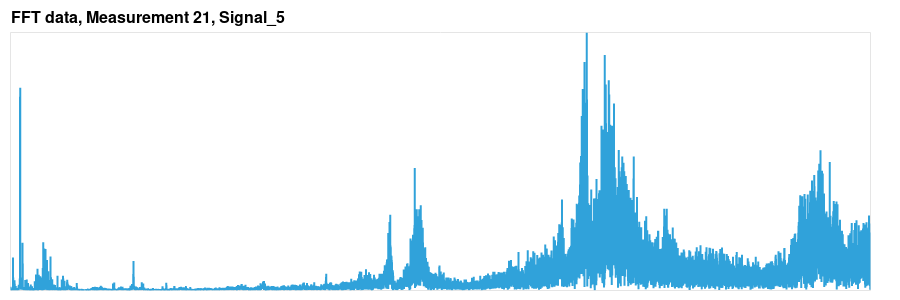
\includegraphics[width=\textwidth]{figures/Signal_5_fft_example.png}
\caption{Signal 5 fft example}
\label{fft_example}
\end{figure}

Es wird sich zeigen, dass der Algorithmus für die dünnbesetzte Hauptkomponentenanalyse sehr rechenintensiv sein kann. Daher haben wir uns entschieden, nur einen Teil der ursprünglichen Zeitreihe zu verwenden. Mithilfe einem Blick auf das Spektrogramm in Abbildung \ref{spectrogram} erkennen wir, dass sich die Frequenzen über den Messzeitraum kaum verändern. Dies ist darauf zurückzuführen, dass der Maschine konstant Material zugeführt wird. Daher können wir die Dimension um einen Faktor $100$ reduzieren ohne wichtige Informationen zu verlieren. Des Weiteren wurden Teile der Frequenzen, welche außerhalb des Frequenzbereichs des jeweiligen Sensors liegen, abgeschnitten. Somit verbleiben wir mit $p \approx 15,000$ Variablen. Um die Varianzen der Frequenzen vergleichbarer zu machen, haben wir die Daten ähnlich wie bei der klassischen Hauptkomponentenanalyse zentriert.

\begin{figure}
\centering
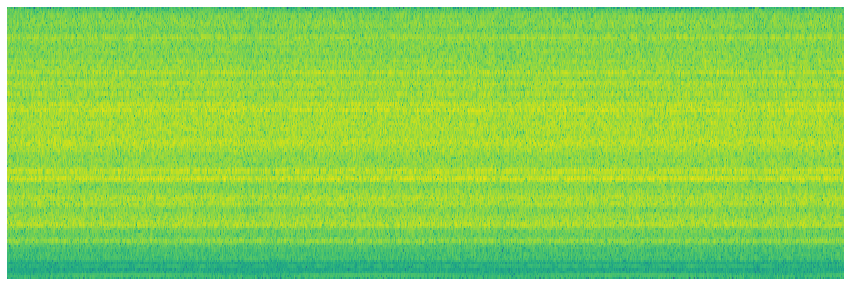
\includegraphics[width=\textwidth]{figures/Signal_5_time_frequency_change.png}
\caption{Signal 5 time frequency change}
\label{spectrogram}
\end{figure}

%----------------------------------------------------------------------------------------
%	Anwedung auf Frequenzdaten
%----------------------------------------------------------------------------------------


\section{Anwendung auf Frequenzdaten}
\label{application_frequency_data}

Unsere Implementierung ermöglicht eine Wahl verschiedene Parameter bezüglich des Modells bzw. des Algorithmus. Für eine Beschränkung der Laufzeit setzen wir eine maximale Anzahl an Iterationen von $500$ und eine Toleranz von $10^{-4}$. Falls nach $500$ Iterationen die vorgegebene Toleranz noch immer nicht erreicht ist, werden wir dies im Folgenden kenntlich machen. Ein Modellparameter, den es zu wählen gilt, ist die Anzahl zu berechnender Hauptkomponenten. Wie bereits in \ref{spca_theorems} beschrieben, wird dazu meist das Ergebnis einer klassischen Hauptkomponentenanalyse verwendet. Es hat sich gezeigt, dass $2$ Hauptkomponenten für die meisten Sensoren ausreichen, um einen Großteil des Datensatzes zu erklären. Zu Analysezwecken haben wir uns dennoch entschieden einen Durchlauf mit $2$ und einen mit $10$ Hauptkomponenten zu starten. 

Interessanter ist die Wahl der Hyperparameter $\lambda$ und $\alpha$, welche wesentlichen Einfluss auf die Ergebnisse besitzen. Auch wenn prinzipiell die Möglichkeit besteht, differenzierte Bestrafungen je Hauptkomponente $\lambda_j$ auszuwählen, beschränken wir uns der Einfachheit halber auf eine einheitliche Bestrafung. Für die Wahl von $\lambda$ haben wir sowohl mehrere Werte ausprobiert, als auch eine Rastersuche bezüglich der in \ref{choice_of_tuning_parameters} beschriebenen BIC-Kriterien durchgeführt. Dafür verwenden wir auf einer log-Skala gleichverteilte Werte im Bereich zwischen $10^{-7}$ und $10^0$. Dagegen wählen wir für das Verhältnis zwischen Lasso und Ridge-Bestrafung die Werte $[0.1,\, 0.5,\, 0.7,\, 0.9,\, 0.95,\, 0.99,\, 1]$. Mithilfe des BIC-Kriteriums können wir zeitgleich über $\lambda$ und $\alpha$ optimieren. Es hat sich in den Anwendungen gezeigt, dass eine geeignete Liste für $\alpha$ mehr Werte nahe $1$ hat, da sich dort die größten Änderungen ergeben. Damit stärken wir den Lasso-Strafterm im Vergleich zum Ridge-Strafterm.

Exemplarisch werden wir uns nun mit einem der Beschleunigungssensoren weiter beschäftigen. An dieser Stelle möchten wir erwähnen, dass wir die Sensoren getrennt betrachten, d.h. die dünnbesetzte Hauptkomponentenanalyse auf die Sensoren einzeln anwenden. Dies ist aufgrund der Unterschiedlichkeit der Sensoren sinnvoll. Wir werden nun ausgewählte Ergebnisse vorstellen. 


%----------------------------------------------------------------------------------------
%	Auswertung der Ergebnisse
%----------------------------------------------------------------------------------------


\section{Auswertung der Ergebnisse}
\label{evaluation}

Im Rahmen dieser Arbeit können wir nun einen begrenzten Teil der Ergebnisse präsentieren. Ziel wird es sein, wesentliche Ergebnisse und Effekte des Algorithmus zu erläutern und gegebenenfalls weiter ins Detail zu gehen. 


%----------------------------------------------------------------------------------------
%	Klassische Analyse der Hauptachsen
%----------------------------------------------------------------------------------------


\subsection{Klassische Analyse der Hauptachsen}

Zunächst wollen wir eine klassische Analyse durchführen, wie sie oft für ein derartiges Verfahren gemacht wird. Um einen Vergleich zu ermöglichen, haben wir sowohl die klassische als auch die dünnbesetzte Hauptkomponentenanalyse durchgeführt. 

Für einen ersten Einblick in die Ergebnisse betrachten wir Abbildung \ref{sparse_pca_classical_analysis_pc_graph} bzw. \ref{sparse_pca_classical_analysis_sparse_pc_graph}, in welcher die ersten beiden Hauptkomponenten gegeneinander aufgezeichnet sind. Dies ist die Darstellung der Daten bezüglich der neu gefundenen Variablen. Zuerst wenden wir uns den Ergebnissen der klassischen Hauptkomponentenanalyse zu. Man sieht schnell, dass sich vier Gruppierungen ergeben. Durch die Transformation sehen wir eine deutliche Trennung zwischen Messungen mit und ohne Material, welche im Bild durch verschiedene Farben markiert sind. Des Weiteren sind die Messungen mit bzw. ohne Material in zwei Untergruppen geteilt. Die Unterschiede sind auf verschiedene Betriebszustände der Maschine zurückzuführen, auf welche wir hier nicht genauer eingehen können. Vergleichen wir dieses Ergebnis mit der dünnbesetzten Variante in Abbildung \ref{sparse_pca_classical_analysis_sparse_pc_graph}, erkennen wir viele Gemeinsamkeiten. Es treten dieselben Gruppierungen wie zuvor auf, so dass noch immer eine Trennung der Messungen bezüglich der Befüllung möglich ist. Ein kleinerer Unterschied ist in der zweiten Hauptkomponenten zu sehen, da bei der dünnbesetzten Variante drei Messungen noch stärker separiert werden.

Nun gilt es, das Zustandekommen dieses Bildes zu erklären. Wir wollen verstehen, warum wir eine Trennung zwischen Messungen bezüglich der Befüllung sehen. Vor allem interessieren wir uns dafür, welche Frequenzen für diesen Unterschied verantwortlich sind. Zu diesem Zweck betrachten wir Abbildung \ref{sparse_pca_classical_analysis_principal_axis} bzw. \ref{sparse_pca_classical_analysis_sparse_principal_axis}, in welcher die Hauptachsen der beiden Varianten zu sehen sind. Anhand der Hauptachsen können wir erkennen, welche Frequenzen eine entscheidende Rolle bei der Erhaltung der maximalen Varianz spielen. Demnach sind die größten Unterschiede im Datensatz auf die Frequenzen mit der größten Amplitude zurückzuführen. Auch wenn es in den niederen Frequenzen nicht leicht zu erkennen ist, sind bei der klassischen Hauptachse alle $\approx 15,000$ Einträge von Null verschieden sind. Eine Erklärung der beschriebenen Effekte ist hier quasi unmöglich. Wir können lediglich aussagen, dass die höheren Frequenzen in einer gewissen Weise wichtig sind. Genau hier liegt das Problem der klassischen Variante, denn eine Interpretation der Hauptachsen ist selten möglich. Es fließen einfach zu viele Koeffizienten in das Modell ein. Dagegen reduziert sich bei der dünnbesetzten Variante die Anzahl von Null verschiedener Einträge auf $\approx 40$ für $\lambda = 0.1$ und $\alpha = 0.1$. Durch die eingeschränkte Modellkomplexität erkennen wir drei Peaks im Frequenzspektrum. Im Wesentlichen sind also nur viel weniger Frequenzen für die beschriebene Trennung verantwortlich. Daher können wir folgern, dass genau diese Frequenzen durch die Maschine verursacht werden. Mit diesem Verfahren ist es also möglich Frequenzen zu identifizieren, welche eine klare Bedeutung im Kontext besitzen.

Zuletzt betrachtet man Abbildung \ref{sparse_pca_classical_analysis_scree_plot}, welche einen sog. \textit{scree plot} zeigt und oft als Bewertungsmittel von Dimensionsreduktionsverfahren dient. Mithilfe dieses Bildes kann man einsehen, welchen Anteil der Varianz des Datensatzes mit der niedrigdimensionalen Repräsentation erklärt wird. Zur Verdeutlichung der Effekte haben wir $10$ Hauptkomponenten berechnet. Es zeichnet sich ein klarer Varianzverlust je Hauptkomponente ab, wenn wir die dünnbesetzte Hauptkomponentenanalyse nutzen. Hier erhalten wir nur $25$\% der Information des Datensatz, während es im Gegensatz dazu $95$\% bei der klassischen Variante sind. Besonders deutlich wird der Kompromiss, den wir eingehen müssen. Dadurch, dass unsere Hauptachsen einfacher zu interpretieren sind, verlieren wir an erklärter Varianz. Ein geeignetes Maß zwischen Modellkomplexität und Rekonstruktionsfehler zu finden, kann von der Anwendung und der Intention abhängen. In unserem Fall ist die Möglichkeit einer Interpretation der Hauptachsen deutlich wichtiger als die Varianzerhaltung. Wir haben durch Abbildung \ref{sparse_pca_classical_analysis_pc_graph} bzw. \ref{sparse_pca_classical_analysis_sparse_pc_graph} gesehen, dass uns durch einen Rückgang der Varianz nicht zwangsläufig Informationen verloren gehen müssen. Wir konnten trotz geringer Varianz ein ähnliches Bild mit denselben Gruppierungen erzielen.

\begin{figure}
\centering
\begin{subfigure}{0.45\textwidth}
\centering
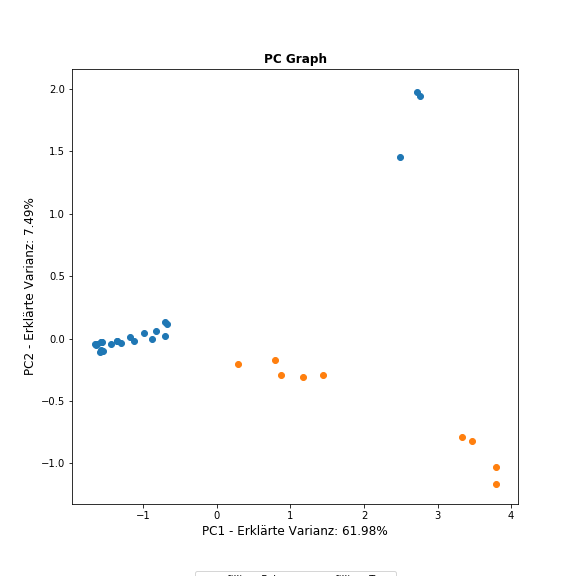
\includegraphics[width = \textwidth]{figures/Signal_5_pc_graph.png}
\caption{Signal 5 PC Graph}
\label{sparse_pca_classical_analysis_pc_graph}
\end{subfigure}
%
\begin{subfigure}{0.45\textwidth}
\centering
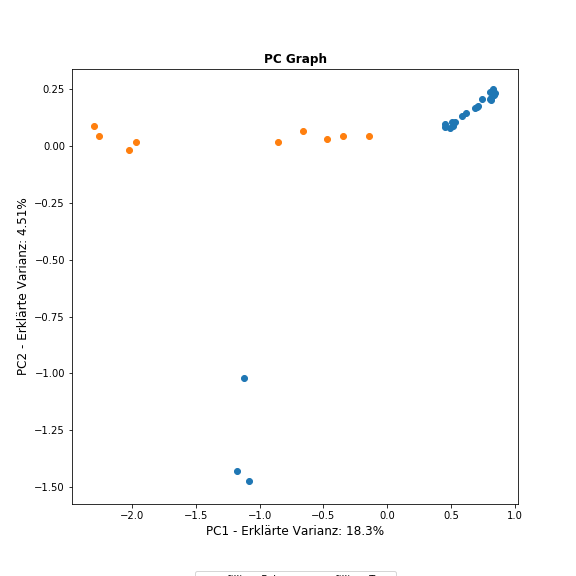
\includegraphics[width = \textwidth]{figures/Signal_5_sparse_pc_graph.png}
\caption{Signal 5 Sparse PC Graph}
\label{sparse_pca_classical_analysis_sparse_pc_graph}
\end{subfigure}
%
\begin{subfigure}{0.9\textwidth}
\centering
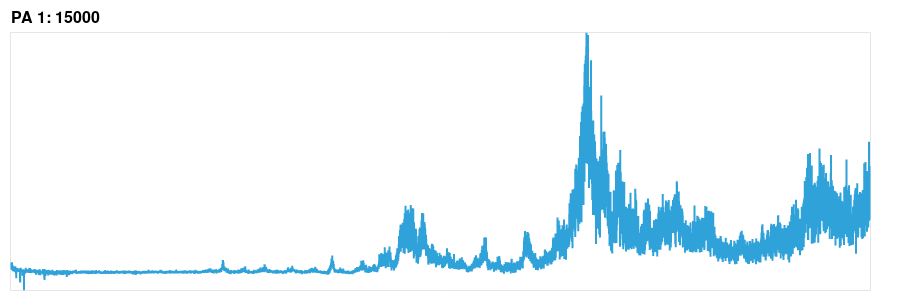
\includegraphics[width=\textwidth]{figures/Signal_5_principal_axis.png}
\caption{Signal 5 principal axis}
\label{sparse_pca_classical_analysis_principal_axis}
\end{subfigure}
%
\begin{subfigure}{0.9\textwidth}
\centering
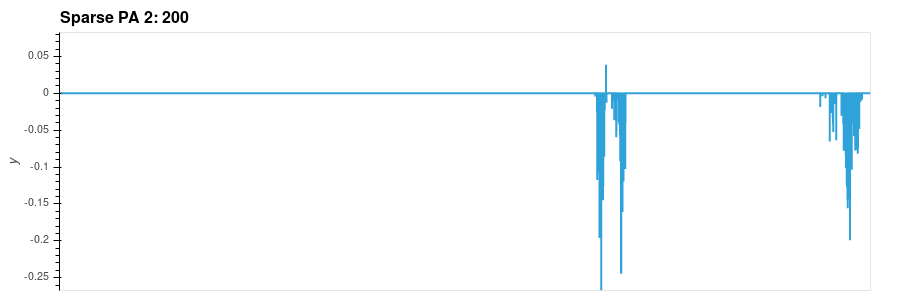
\includegraphics[width=\textwidth]{figures/Signal_5_sparse_principal_axis.png}
\caption{Signal 5 sparse principal axis}
\label{sparse_pca_classical_analysis_sparse_principal_axis}
\end{subfigure}
%
\begin{subfigure}{0.9\textwidth}
\centering
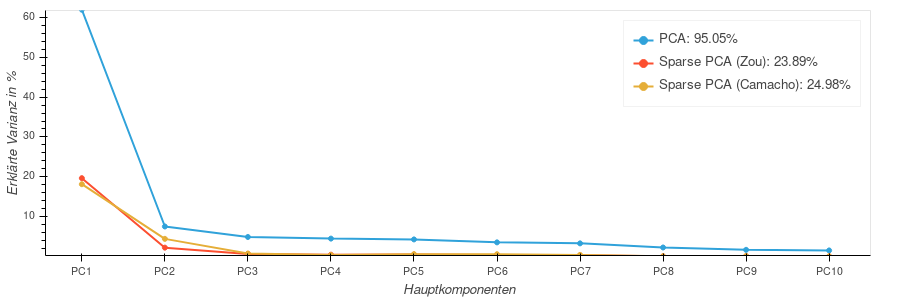
\includegraphics[width = \textwidth]{figures/Signal_5_scree_plot_10.png}
\caption{Signal 5 Scree Plot}
\label{sparse_pca_classical_analysis_scree_plot}
\end{subfigure}
\caption{Vergleich der klassischen mit der dünnbesetzten Hauptkomponentenanalyse für $\lambda=10^{-4}$ und $\alpha = 0.95$.}
\label{sparse_pca_classical_analysis}
\end{figure}


%----------------------------------------------------------------------------------------
%	Wahl der Hyperparameter
%----------------------------------------------------------------------------------------


\subsection{Wahl der Hyperparameter}

Im vorangegangenem Abschnitt haben wir beispielhaft gezeigt, wie die Ergebnisse einer dünnbesetzten Hauptkomponentenanalyse zu interpretieren sind. Für die Analyse haben wir bestimmte Werte von $\alpha$ und $\lambda$ vorgegeben, die möglichst gute Ergebnisse erzielen. Es stellt sich jedoch die Frage, wie sich die einzelnen Hauptachsen und Hauptkomponenten verändern, falls wir andere Werte für die Hyperparameter wählen. Zu diesem Zweck wenden wir uns Abbildung \ref{results_parameter_benchmark} zu. Hier haben wir die Anzahl an Hauptkomponenten fixiert und versucht, die Effekte in Abhängigkeit von $\lambda$ für einen akustischen Sensor zu beschreiben.

Abbildung \ref{results_parameter_benchmark_degrees_of_freedom} zeigt wie sich $\operatorname{df}(\lambda)$, also die Anzahl von Null verschiedener Einträge in den Hauptachsen, bei Veränderung von $\lambda$ bzw. $\alpha$ verhält. Klar erkennbar ist der relativ gleichmäßige Abfall der Freiheitsgrade, d.h. für wachsendes $\lambda$ werden unsere Hauptachsen zunehmend dünnbesetzt. Dies entspricht unseren Erwartungen aus Kapitel \ref{sparse_pca}. Verschieben wir das Verhältnis der Bestrafung von der $\ell_1$ zur $\ell_2$-Norm, sprich kleineres $\alpha$, steigt die Anzahl der Freiheitsgrade. Dies bestätigt, dass die $\ell_1$-Norm im Gegensatz zur $\ell_2$-Norm eine Dünnbesetzung hervorruft. Ab einem gewissem Punkt $\lambda \approx 10^{-2}$ für $\alpha > 0.5$ bzw. $\lambda \approx 10^{-1}$ für $\alpha = 0.1$ ist die Bestrafung zu stark, so dass die Hauptachsen dem Nullvektor entsprechen und keine Anpassung an den Datensatz mehr stattfindet.

Interessant ist nun, wie sich die erklärte Varianz des Datensatzes im Vergleich verhält, welche in Abbildung \ref{results_parameter_benchmark_explained_variance} zu sehen ist.  Auffällig ist, dass sich für $\lambda$ im Bereich von $[10^{-7}, 10^{-3}]$ kaum Änderungen in der Varianz ergeben. In diesem Bereich sind wir nur leicht unter dem Niveau der klassischen Variante. Im Umkehrschluss können wir aufgrund der kontinuierlichen Stagnation der Freiheitsgrade die Modellkomplexität verringern, aber zeitgleich den Rekonstruktionsfehler auf konstantem Niveau halten. Erst nahe $\lambda \approx 10^{-2}$ für $\alpha > 0.5$ bzw. bei $\lambda \approx 10^{-1}$ für $\alpha = 0.1$ zeichnet sich ein deutlicher Einbruch ab. Dieser ist dadurch zu erklären, dass die Hauptachsen dann dem Nullvektor entsprechen. Aus der Kombination der beiden Abbildungen können wir schließen, dass nur wenige Frequenzen wirklich wichtig zur Erklärung der Varianz des Datensatzes notwendig sind.

Um eine automatisierte Wahl von $\lambda$ und $\alpha$ zu ermöglichen, haben wir in Abschnitt \ref{choice_of_tuning_parameters} Vorgehensweisen mithilfe eines BIC-Kriteriums beschrieben. Eine Anwendung des Kriteriums nach \cite{croux, guo} befindet sich in Abbildung \ref{results_parameter_benchmark_bic}. Hier zeichnet sich ein Minimum im Bereich von $\lambda \in [10^{-4}, 10^{-3}]$ für $\alpha > 0.5$ bzw. nahe $\lambda \approx 10^{-2}$ ab, welches wir nach obiger Analyse erwarten konnten. Es wird also ein Punkt gewählt, an welchem die erklärte Varianz gerade noch auf sehr hohem Niveau, aber die Modellkomplexität gering ist. Letztere Abbildung ist also eine Kombination der Erkenntnisse und kann genutzt werden, um eine Balance zwischen Dünnbesetzung und erklärter Varianz zu finden. An dieser Stelle möchten wir erwähnen, dass die Resultate des BIC-Kriteriums nicht für alle Sensoren zufriedenstellend waren. Genauer gesagt sehen wir in manchen Fällen, dass die Gewichtung zwischen Modellkomplexität und Rekonstruktionsfehler nicht passend gewählt ist. Dies kann daran liegen, dass BIC-Kriterien in hochdimensionalen Fällen versagen können \cite{giraud}. Für unsere Zwecke wurden für die betroffenen Sensoren daher eine manuelle Gewichtung vorgenommen.

\begin{figure}
\centering
\begin{subfigure}{0.9\textwidth}
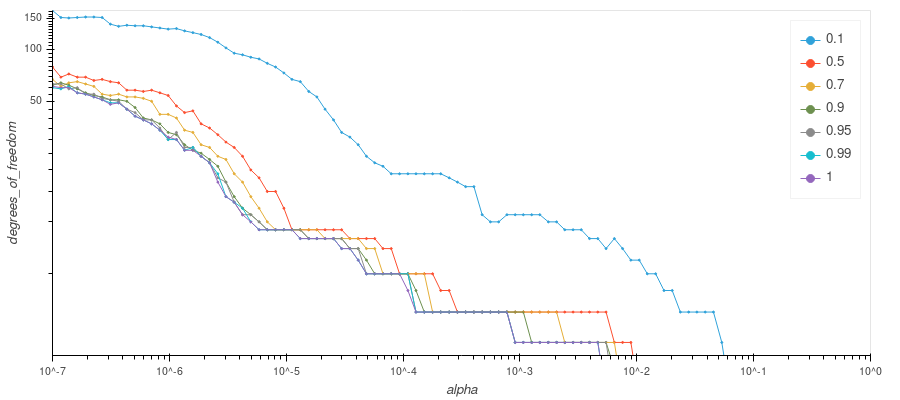
\includegraphics[width=\textwidth]{figures/Signal_0_degrees_of_freedom.png}
\caption{Anzahl Freiheitsgrade in Abhängigkeit von $\lambda$.}
\label{results_parameter_benchmark_degrees_of_freedom}
\end{subfigure}
%
\begin{subfigure}{0.9\textwidth}
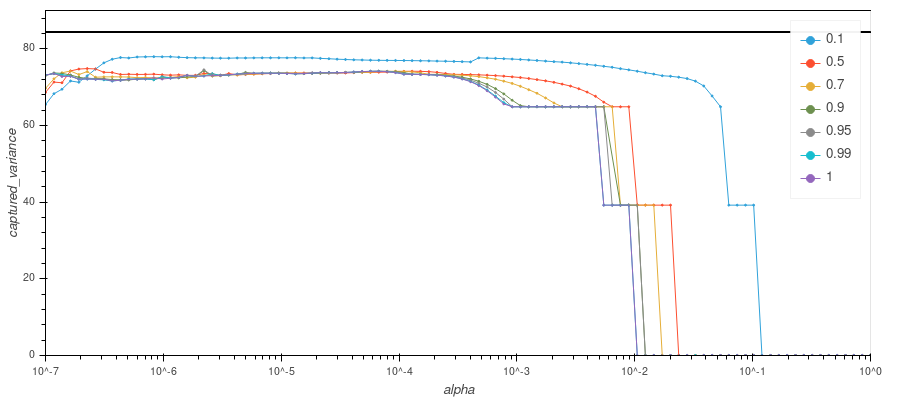
\includegraphics[width=\textwidth]{figures/Signal_0_explained_variances.png}
\caption{Erklärte Varianz des Datensatzes in Abhängigkeit von $\lambda$.}
\label{results_parameter_benchmark_explained_variance}
\end{subfigure}
%
\begin{subfigure}{0.9\textwidth}
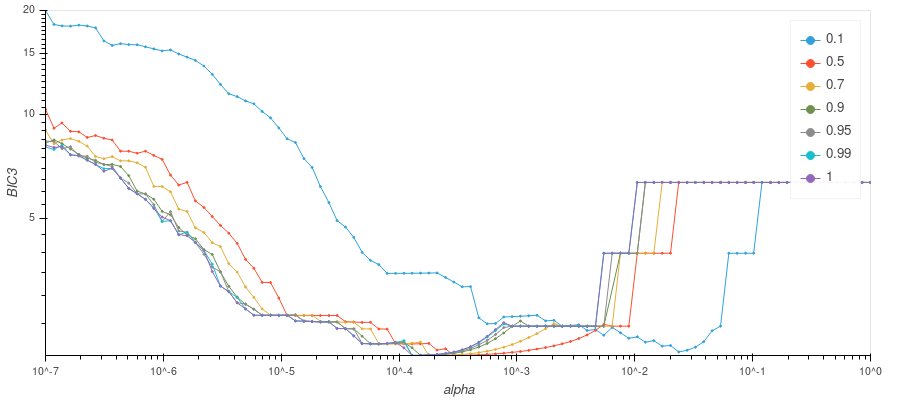
\includegraphics[width=\textwidth]{figures/Signal_0_bic.png}
\caption{Wahl der Hyperparameter mithilfe eines minimalen BIC-Kriteriums.}
\label{results_parameter_benchmark_bic}
\end{subfigure}
\caption{Die Abbildung zeigt wie sich eine Wahl der Hyperparameter $\alpha$ und $\lambda$ mithilfe eines BIC-Kriterium gestalten kann. Um Erkenntnisse über die Entstehung der BIC-Abbildung zu gewinnen, werden zusätzlich die beiden Komponenten Anzahl Freiheitsgrade und erklärte Varianz gezeigt. Zu beachten ist die logarithmische Skala für $\lambda$.}
\label{results_parameter_benchmark}
\end{figure}


%----------------------------------------------------------------------------------------
%	Verhalten des Algorithmus
%----------------------------------------------------------------------------------------


\subsection{Verhalten des Algorithmus}

Im Zuge dieser Arbeit möchten wir nicht nur die Ergebnisse einiger Experimente, sondern auch das Verhalten des Algorithmus an sich beschreiben. Dafür werden wir uns verschiedene Größen wie Laufzeit, Anzahl Iterationen und Toleranz ansehen. Um ein Gefühl für diese Größen bei der dünnbesetzten Hauptkomponentenanalyse zu bekommen, haben wir einen Überblick in Tabelle \ref{algorithm_analysis_table} erstellt. Interessant dabei ist vor allem die Abhängigkeit vom Hyperparameter $\lambda$. Je kleiner wir die Bestrafung wählen, desto länger dauert der Algorithmus und desto mehr Iterationen werden benötigt. Da bei kleinem $\lambda$ mehr von Null verschiedene Einträge in den Hauptachsen erlaubt werden, stimmt diese Beobachtung mit der Komplexität des Algorithmus von Abschnitt \ref{complexity} überein. Die meiste Zeit wird dabei nicht überraschend für das Lösen des Elastic Nets durch das Koordinatenabstiegsverfahren verwendet. Hingegen sind die Kosten für das Minimieren über $\mat A$ unabhängig von den Hyperparametern und im Wesentlichen durch eine Singulärwertzerlegung bestimmt, welche für diesen Datensatz in einem Bruchteil einer Sekunde gelöst werden kann. Ein Blick auf Tabelle REF zeigt die Ergebnisse eines Profilers und bestätigt unsere Erwartungen.

\setlength{\tabcolsep}{12pt}
\begin{table}
\centering
\begin{tabular}{cccc}
$\bm{\lambda}$ & \textbf{Laufzeit} & \textbf{Iterationen} & \textbf{Toleranz}\\\hline\addlinespace
$10^{-6}$ & $65235.76$ sec & $>500$ & $2.271780 \cdot 10^{-1}$\\
$10^{-5}$ & $9158.24$ sec & $>500$ & $4.132993 \cdot 10^{-4}$\\
$10^{-4}$ & $777.36$ sec & $99$ & $4.233382 \cdot 10^{-5}$\\
$10^{-3}$ & $201.49$ sec & $54$ & $5.531939 \cdot 10^{-5}$\\
$10^{-2}$ & $20.19$ sec & $5$ & $0$\\
$10^{-1}$ & $4.65$ sec & $1$ & $0$\\
\end{tabular}
\caption{Die Tabelle gibt einen Überblick über die Veränderung von Laufzeit, Iteration und Toleranz in Abhängigkeit von $\lambda$. Dabei wurde $\alpha=0.5$ und die Anzahl an Hauptkomponenten $k=10$ fest gewählt.\\Gerechnet wurde auf einem Intel Xeon Gold 6130F@2.10GHz.}
\label{algorithm_analysis_table}
\end{table}
\setlength{\tabcolsep}{6pt}

Logischerweise erhöht sich mit der Anzahl an Iterationen auch die Laufzeit des Algorithmus. Aus Tabelle \ref{algorithm_analysis_table} lässt sich aber nicht direkt erkennen, ob sich auch die Laufzeit je Iteration mit $\lambda$ verändert. In Abbildung \ref{run_time_per_iteration} beobachten wir auch eine Zunahme der Laufzeit je Iteration bei Senkung von $\lambda$ im Mittel. Des Weiteren steigt die Laufzeit, wenn mehr Gewicht auf eine Lasso-Bestrafung gelegt wird, also $\alpha$ nahe 1 gewählt wird.

Da wir eine maximale Anzahl von $500$ Iterationen festgelegt haben, kommt es bei Werten $\lambda < 10^{-5}$ zu einer erhöhten Toleranz. Eine Erhöhung der Anzahl an Iterationen kann die Toleranz verringern, jedoch steigt damit auch die Laufzeit. Diese Obergrenze scheint für unsere Anwendung eine sinnvolle Wahl zu sein, muss aber für jeden Datensatz geeignet angepasst werden. Denkbar sind auch schwächere Konvergenzkriterien, die gegebenenfalls die Laufzeit verringern können.

\begin{figure}
\centering
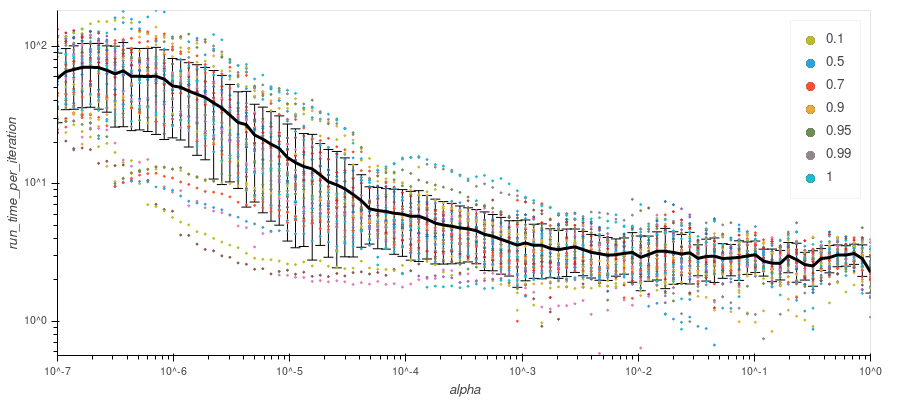
\includegraphics[width = 0.9\textwidth]{figures/run_time_per_iteration.png}
\caption{In dieser Abbildung ist die Laufzeit pro Iteration bei Veränderung des Hyperparameters $\lambda$ auf einer logarithmischen Skala zu sehen. Da auch $\alpha$ in unseren Experimenten variiert worden ist und mehrere Sensoren betrachtet werden, sehen wir mehrere Punkte je $\lambda$. Im Mittel klar zu erkennen ist ein Anstieg der Laufzeit bei Verringerung der Stärke der Bestrafung $\lambda$.}
\label{run_time_per_iteration}
\end{figure}


%----------------------------------------------------------------------------------------
%	Experimentelle Überprüfung der berechneten Varinanz
%----------------------------------------------------------------------------------------


\subsection{Experimentelle Überprüfung der berechneten Varianzen}

In Abschnitt \ref{adjustment_of_variances} haben wir unterschiedliche Wege zur Berechnung der Hauptkomponenten und deren erklärte Varianz gezeigt. Um die Arbeit von Camacho et al. \cite{camacho} experimentell zu überprüfen, werden wir vier Kriterien definieren, welche auf den unterschiedlichen Vorgehensweisen basieren. Für jede dieser wird die Varianz der Residuen addiert und mit der Gesamtvarianz des Datensatzes normalisiert.
\begin{itemize}
\item TotQR: $\quad \frac{\sum_{j=1}^k R_{jj}^2 + \spur{\mat E^T\mat E}}{\spur{\mat X^T\mat X}} \quad$ (Vorgehensweies Zou et al.)
\item TotZB: $\quad \frac{\spur{\mat B \mat Z^T \mat Z \mat B^T} + \spur{\mat E^T\mat E}}{\spur{\mat X^T\mat X}} \quad$ (Vorgehensweise Camacho et al.)
\end{itemize}
Bezüglich der Notation haben wir uns an Abschnitt \ref{adjustment_of_variances} gehalten. Zwei weitere Kriterien TotQR* und TotZB* ergeben sich durch die Korrektur der Hauptkomponenten mit der Moore-Penrose-Inverse $\mat Z^* = \mat X \mat B^T (\mat B^T\mat B)^+$. Falls alle Vorgehensweisen korrekt sind, können wir erwarten, dass jedes Kriterium den Wert $1$ hat. In Abbildung \ref{total_variance_validation} haben wir die Kriterien für unsere Experimente berechnet. Klar zu sehen ist, dass ohne eine Korrektur mit der Moore-Penrose-Inversen beide Varianten für die Varianzberechnung im Allgemeinem falsch sind. Auch wenn wir die Hauptkomponenten korrigieren, liefert die QR-Zerlegung keine richtigen Ergebnisse. Nur TotZB* hat in allen Fällen den Wert $1$ und ist damit der einzig korrekte Weg, Hauptkomponenten und Varianzen zu berechnen. Die von Zou et al. \cite{zou_sparsepca} vorgeschlagenen Varianten sind also falsch und sollten nicht verwendet werden. Somit können wir die Erkenntnisse aus \cite{camacho} experimentell bestätigen.

\begin{figure}
\centering
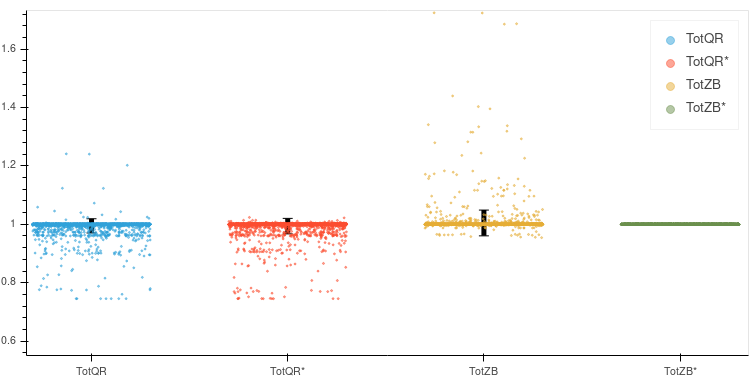
\includegraphics[width = 0.9\textwidth]{figures/total_variance_validation.png}
\caption{Zu sehen sind die Ergebnisse der unterschiedlichen Vorgehensweise bei der Berechnung der Hauptkomponenten und erklärter Varianzen. Nur die von Camacho et al. vorgeschlagene Variante TotZB* errechnet diese korrekt. Jeder Punkt entspricht eines unserer Experimente wie in Abschnitt \ref{application_frequency_data} beschrieben.}
\label{total_variance_validation}
\end{figure}